\chapter{Karush-Kuhn-Tucker conditions}
\label{chap:kkt_conditions}

In this chapter, we will explore conditions which characterize solutions in
constrained optimization problems, the most well-known being a set of conditions
known as the Karush-Kuhn-Tucker (KKT) conditions. This flows naturally from our 
study of Lagrange duality in the last chapter. In fact, the last chapter already
established a key relationship between primal and dual solutions and what 
are called saddle points of the Lagrangian. These arguments were given in 
passing and below we revisit them as they will lay the foundation for the KKT 
conditions, which we will cover subsequently.        

\section{Saddle point condition}
\label{sec:saddle_point_condition}

As in the last chapter, consider a primal problem
\begin{equation}
\label{eq:primal_problem2}
\begin{alignedat}{2}
&\minimize_x \quad && f(x) \\
&\st \quad && h_i(x) \leq 0, \; i=1,\dots,m \\ 
& && \ell_j(x) = 0, \; j=1,\dots,k,
\end{alignedat}
\end{equation}
whose associated Lagrangian and dual function are
\begin{align*}
L(x,u,v) &= f(x) + \sum_{i=1}^m u_i h_i(x) + \sum_{j=1}^k v_j \ell_j(x), \\ 
g(u,v) &= \inf_x \, L(x,u,v), 
\end{align*}
and whose associated dual problem is 
\begin{equation}
\label{eq:dual_problem2}
\maximize_{u,v} \quad g(u,v) \quad \st \quad u \geq 0.
\end{equation}
We do not assume that \eqref{eq:primal_problem2} is convex, though recall, the 
dual problem \eqref{eq:dual_problem2} is always convex. In general, we say that
a triplet \smash{$\bar{x}, \bar{u}, \bar{v}$} is a \emph{saddle point} of the
Lagrangian if  
\index{Lagrangian function!saddle point} 
\begin{equation}
\label{eq:lagrangian_saddle_point2}
L(\bar{x}, u, v) \leq L(\bar{x}, \bar{u}, \bar{v}) \leq L(x, \bar{u}, \bar{v}),
\quad \text{for any $x$ and any $u \geq 0, \, v$}.
\end{equation}
In other words, starting at \smash{$\bar{x}, \bar{u}, \bar{v}$}, the condition
says: if we move the primal variable away from \smash{$\bar{x}$} then $L$ can
only increase; if we move the dual variables away from \smash{$\bar{u},
  \bar{v}$}, then $L$ can only decrease.    

The following is a useful characterization of primal and dual solutions via
saddle points.  

\begin{Theorem}
\label{thm:saddle_point_optimality}
For any primal problem \eqref{eq:primal_problem2} and its dual
\eqref{eq:dual_problem2}, and any primal feasible \smash{$\bar{x}$} and dual
feasible \smash{$\bar{u}, \bar{v}$}, the triplet \smash{$\bar{x}, \bar{u},
  \bar{v}$} is a saddle point of the Lagrangian
\eqref{eq:lagrangian_saddle_point2} if and only if \smash{$\bar{x}$} is primal
optimal, \smash{$\bar{u}, \bar{v}$} are dual optimal, and strong duality holds. 
\end{Theorem}

Though the arguments behind this result were already given in Chapter 
\ref{chap:lagrangian_duality}, it will be helpful to consolidate them here.
First, note that the saddle point condition
\eqref{eq:lagrangian_saddle_point2} has a couple of equivalent forms:
\begin{equation}
\label{eq:lagrangian_saddle_point3}
\sup_{u \geq 0, \, v} \, L(\bar{x}, u, v) = L(\bar{x}, \bar{u}, \bar{v}) =
\inf_x \, L(x, \bar{u}, \bar{v}), 
\end{equation}
as well as
\begin{equation}
\label{eq:lagrangian_saddle_point4}
f(\bar{x}) = L(\bar{x}, \bar{u}, \bar{v}) = g(\bar{u}, \bar{v}).
\end{equation}
The right-hand side in the above display is due to the definition of the dual
function $g$, whereas the left-hand side uses the representation of $f$ as a
supremum of the Lagrangian, from Property \parref{par:max_min}. To prove    
Theorem \ref{thm:saddle_point_optimality} we simply observe that 
\eqref{eq:lagrangian_saddle_point4} is equivalent to \smash{$\bar{x}, \bar{u}, 
  \bar{v}$} being primal and dual solutions with zero duality gap. 

\section{Karush-Kuhn-Tucker conditions}
\label{sec:kkt_conditions}

We say that a triplet \smash{$\bar{x}, \bar{u}, \bar{v}$} is a
\emph{Karush-Kuhn-Tucker (KKT) point} associated with the primal and 
dual pair \eqref{eq:primal_problem2} and \eqref{eq:dual_problem2} if it
satisfies the following conditions: 
\index{KKT conditions}
\begin{alignat}{2}
\label{eq:kkt_stationarity}
&0 \in \partial_x L(\bar{x}, \bar{u}, \bar{v}) \quad
&& \text{(stationarity)} \\
\label{eq:kkt_complementary_slackness} 
&\bar{u}_i h_i(\bar{x}) = 0, \; i = 1,\dots,m \quad 
&& \text{(complementary slackness)} \\
\label{eq:kkt_primal_feasibility}
&h_i(\bar{x}) \leq 0, \; i = 1,\dots,m, \; \text{and} \; 
\ell_j(\bar{x}) = 0, \; j = 1,\dots,k \quad 
&& \text{(primal feasibility)} \\ 
\label{eq:kkt_dual_feasibility}
&\bar{u}_i \geq 0, \; i = 1,\dots,m. \quad
&& \text{(dual feasibility)}
\end{alignat}
To be clear, in \eqref{eq:kkt_stationarity}, called the stationarity condition,
the subdifferential is taken with respect to the $x$ component of the
Lagrangian.  

The next result shows that the KKT conditions offer yet another equivalent
characterization of saddle point condition (together with feasibility).  

\begin{Lemma}
\label{lem:saddle_point_kkt}
For any primal feasible \smash{$\bar{x}$} and dual feasible \smash{$\bar{u}, 
  \bar{v}$}, the saddle point condition \eqref{eq:lagrangian_saddle_point2} is
equivalent to stationarity and complementary slackness,
\eqref{eq:kkt_stationarity} and \eqref{eq:kkt_complementary_slackness}.
\end{Lemma}

The proof is straightforward, if we use the equivalent form of the saddle point
condition \eqref{eq:lagrangian_saddle_point4}. The second equality in
\eqref{eq:lagrangian_saddle_point4} is equivalent to the fact that
\smash{$\bar{x}$} minimizes \smash{$L(\cdot, \bar{u}, \bar{v})$}, which is
equivalent to stationarity \eqref{eq:kkt_stationarity}. The first equality in
\eqref{eq:lagrangian_saddle_point4} is implied by complementary slackness
\eqref{eq:kkt_complementary_slackness}:
\[
L(\bar{x}, \bar{u}, \bar{v}) = f(\bar{x}) + 
\sum_{i=1}^m \underbrace{\bar{u}_i h_i(\bar{x})}_{=\,0} + 
\sum_{j=1}^k \underbrace{\bar{v}_j \ell_j(\bar{x})}_{=\,0} 
= f(\bar{x}),
\]
where we have used primal feasibility. Furthermore, the first equality in
\eqref{eq:lagrangian_saddle_point4} also implies complementary slackness: if
\smash{$f(\bar{x}) = L(\bar{x}, \bar{u}, \bar{v})$}, then (again using primal
and dual feasibility) we conclude that all summands must be zero in the middle
expression of the last display, which leads to
\eqref{eq:kkt_complementary_slackness}. This completes the proof the theorem.

Combining Theorem \ref{thm:saddle_point_optimality} and Lemma
\ref{lem:saddle_point_kkt} yields the following important result. 

\begin{Theorem}
\label{thm:kkt_optimality}
For any primal problem \eqref{eq:primal_problem2} and its dual
\eqref{eq:dual_problem2}, a triplet \smash{$\bar{x}, \bar{u}, \bar{v}$}
satisfies the KKT conditions
\eqref{eq:kkt_stationarity}--\eqref{eq:kkt_dual_feasibility} if and only if 
\smash{$\bar{x}$} is primal optimal, \smash{$\bar{u}, \bar{v}$} are dual
optimal, and strong duality holds. In other words, the KKT conditions are always
sufficient for optimality, and necessary under strong duality.   
\end{Theorem}

\index{KKT conditions!optimality}
\index{subgradient!optimality condition}
\index{Lagrange multiplier condition} 
It is worth noting that the KKT conditions generalize the subgradient optimality
condition \eqref{eq:subgradient_optimality}. That is, if problem
\eqref{eq:primal_problem2} has no constraints ($m = k = 0$), then the Lagrangian
is simply the primal criterion, $L = f$, and the only non-vacuous KKT condition
is stationarity \eqref{eq:kkt_stationarity}, which reduces to
\eqref{eq:subgradient_optimality}. Similarly, the KKT conditions generalize the
Lagrange multiplier condition \eqref{eq:lagrange_multiplier}, which can seen
either because the subgradient optimality condition does, or directly from
stationarity \eqref{eq:kkt_stationarity} with linear equality constraints of the
form $Ax = b$. Exercise \ref{ex:subgradients_kkt} studies further connections.  

\begin{Example}
The following examples discuss the KKT conditions for problems of interest. In
each case, the KKT conditions are necessary and sufficient for optimality, as
the problem in question is convex and strong duality holds by Slater's condition
(Theorem \ref{thm:slater_condition}). 

\begin{enumerate}[label=\alph*., ref=\alph*]
\item Consider a QP with equality constraints only, 
  \begin{alignat*}{2}
  &\minimize_x \quad && c^\T x + \frac{1}{2} x^\T Q x \\
  &\st \quad && Ax = b,
  \end{alignat*}
  where $Q \succeq 0$. Its Lagrangian is 
  \[
  L(x,v) = c^\T x + \frac{1}{2} x^\T Q x + v^\T (Ax - b).
  \]
  Complementary slackness \eqref{eq:kkt_complementary_slackness} and dual
  feasibility \eqref{eq:kkt_dual_feasibility} are vacuous due to the lack of 
  inequality constraints. Stationarity \eqref{eq:kkt_stationarity} and primal
  feasibility \eqref{eq:kkt_primal_feasibility} are each linear equations, which
  can be assembled into one combined linear system:
  \index{KKT matrix}
  \[
  \begin{bmatrix} Q & A^\T \\ A & 0 \end{bmatrix}  
  \begin{bmatrix} x \\ v \end{bmatrix} =
  \begin{bmatrix} -c \\ b \end{bmatrix}.
  \]
  The above matrix is often called the \emph{KKT matrix} associated with our
  original QP. 

\item \parlab{xa:lasso_kkt}
  Consider the lasso problem
  \begin{equation}
  \label{eq:lasso_primal2}
  \minimize_\beta \quad \frac{1}{2} \|y - X \beta\|_2^2 + \lambda \|\beta\|_1, 
  \end{equation}
  for a response vector $y \in \R^n$ and feature matrix $X \in \R^{n \times
    d}$. Since this problem has no constraints, the KKT conditions reduce to  
  stationarity (which, as discussed above, is just the subgradient optimality 
  condition):   
  \index{lasso!optimality conditions}
  \begin{equation}
  \label{eq:lasso_optimality}
  X^\T (y - X\beta) = \lambda s, \quad \text{where $s \in \partial
    \|\beta\|_1$}. 
  \end{equation}
  We will see later, in Chapter \ref{sec:lasso_structure}, that this provides a
  basis for understanding the finer structure of lasso solutions.      
  
\item \parlab{xa:svm_kkt}
  Consider the SVM problem
  \begin{equation}
  \label{eq:svm_primal2}
  \begin{alignedat}{2}
  &\minimize_{\beta_0,\beta,\xi} \quad
  && \frac{1}{2} \|\beta\|_2^2 + C \sum_{i=1}^n \xi_i \\ 
  &\st \quad && y_i (\beta_0 + x_i^\T \beta) \geq 1-\xi_i, \;  i=1,\dots,n \\ 
  & && \xi \geq 0,
  \end{alignedat}
  \end{equation}
  for labels $y_i \in \{ -1, 1\}$ and features $x_i \in \R^d$, $i=1,\dots,n$. 
  Its Lagrangian is
  \[
   L(\beta,\beta_0,\xi,\alpha,u) = 
   \frac{1}{2} \|\beta\|_2^2 + C \sum_{i=1}^n \xi_i +  \sum_{i=1}^n \alpha_i 
   \big(1-\xi_i - y_i (\beta_0 + x_i^\T \beta) \big) - u^\T \xi. 
   \]
  The stationarity condition \eqref{eq:kkt_stationarity} reads
  \index{support vector machine!optimality conditions}
  \begin{equation}
  \label{eq:svm_stationarity}
  \sum_{i=1}^n \alpha_i y_i = 0, \quad 
  \sum_{i=1}^n \alpha_i y_i x_i = \beta, \quad
  \alpha_i + u_i = C, \quad i = 1,\dots,n.
  \end{equation}
  Complementary slackness \eqref{eq:kkt_complementary_slackness} reads   
  \begin{equation}
  \label{eq:svm_complementary_slackness}
    \alpha_i \big(1-\xi_i - y_i (\beta_0 + x_i^\T \beta) \big) = 0, \quad
    u_i \xi_i = 0, \quad i=1,\dots,n. 
  \end{equation}
  Together with primal and dual feasibility, the above two conditions
  characterize SVM solutions; the discussion is continued below to demonstrate
  how they reveal the finer structure of SVM solutions.       
\end{enumerate}
\end{Example}

\section{Primal-dual relationships}

For a primal-dual pair \eqref{eq:primal_problem2}, \eqref{eq:dual_problem2}
which exhibit strong duality, we know (Theorem \ref{thm:kkt_optimality}) that
the KKT conditions are necessary and sufficient for optimality. The stationarity
condition \eqref{eq:kkt_stationarity} allows us to relate primal $x^\star$ and
dual $u^\star, v^\star$ solutions. Rephrased, this condition (evaluated at
$x^\star,  u^\star, v^\star$) simply says that
\index{KKT conditions!primal-dual relationship}
\begin{equation}
\label{eq:kkt_stationarity2}
\text{$x^\star$ minimizes $L(\cdot, u^\star, v^\star)$}.
\end{equation}
As demonstrated in the examples that follow, we can often rearrange
\eqref{eq:kkt_stationarity2} to form what we call a \emph{primal-dual
  relationship}, which is an equation that relates primal and dual solutions.
Moreover, if $L(\cdot, u^\star, v^\star)$ has a unique minimizer, then this
relationship uniquely specifies $x^\star$ in terms of $u^\star, v^\star$.     

Primal-dual relationships can be useful for two main reasons. First, in the case
that it uniquely specifies the primal solution $x^\star$, a primal-dual
relationship enables us to solve the primal \eqref{eq:primal_problem2} via the
dual \eqref{eq:dual_problem2}, which is useful in practice when the latter is
easier solve than the former. Second, a primal-dual relationship can provide an
avenue for inferring properties of solutions. A nice example of this is given
by SVM duality, as studied previously in Example \parref{xa:svm_kkt}. 

\begin{Example}
The SVM stationarity condition \eqref{eq:svm_stationarity}
immediately reveals that the primal solution \smash{$\hbeta$} can be written in
terms of the dual solution via \smash{$\hbeta = \sum_{i=1}^n \halpha_i y_i
  x_i$}. Generally, some coordinates of the dual solution will be equal to zero,
\smash{$\halpha_i = 0$}, by the nonnegativity constraint in \eqref{eq:svm_dual};
the corresponding feature vectors $x_i$ and labels $y_i$ play no role in shaping
\smash{$\hbeta$}, which determines the orientation of the linear SVM
classifier. 

\setlength{\parindent}{\normalparindent}
Meanwhile, the coordinates for which \smash{$\halpha_i \not= 0$} correspond to
what are called \emph{support points} of the SVM classifier. By complementary
slackness \eqref{eq:svm_complementary_slackness}, note that \smash{$\halpha_i
  \not= 0$} can hold only if \smash{$y_i (\hbeta_0 + x_i^\T \hbeta) =
  1-\hat\xi_i$}. Further, by carefully inspecting the interaction of the
complementary slackness and stationarity conditions, we can infer the following 
more precise description: 
\index{support vector machine!primal-dual relationship}
\begin{itemize}
\item if \smash{$\halpha_i \not= 0$} and \smash{$\hat\xi = 0$}, then $x_i$ is on
  the ``edge'' of the margin, \smash{$y_i (\hbeta_0 + x_i^\T \hbeta) = 1$};    
\item if \smash{$\halpha_i \not= 0$} and \smash{$\hat\xi \not= 0$}, then $x_i$
  is on the ``wrong side'' of the margin, \smash{$y_i (\hbeta_0 + x_i^\T \hbeta)
    < 1$}, so \smash{$\hat{u}_i = 0$} by complementary slackness
  \eqref{eq:svm_complementary_slackness}, and \smash{$\halpha_i = C$} by   
  stationarity \eqref{eq:svm_stationarity}.
\end{itemize}
Figure \ref{fig:svm} gives a visualization.
\end{Example}

\begin{figure}[tb]
\centering
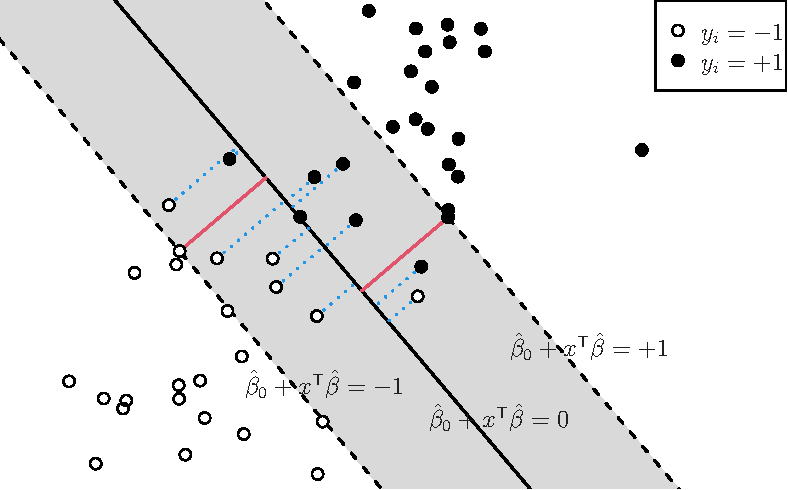
\includegraphics[width=0.7\textwidth]{fig/svm.pdf}
\caption{An example of the SVM classifier. The solid line denotes the
  separating hyperplane, defined by \smash{$\hbeta_0 + x^\T \hbeta = 0$}. There
  are 14 support points (of a total of $n = 50$ samples), corresponding to
  nonzero coordinates of the dual solution \smash{$\halpha$}; for visual 
  emphasis, each one is met by a line segment which runs normal to the
  separating hyperplane. Of the support points, only two are on the ``edge'' of
  the margin, met by the solid line segments.} 
\label{fig:svm}
\end{figure}

For the lasso, as studied in Example \parref{xa:lasso_kkt}, the problem
\eqref{eq:lasso_primal2} has no constraints and thus no associated dual   
variables. As written, the stationarity condition \eqref{eq:lasso_optimality}
relates the primal solution to itself, and not to dual variables. In order to
make progress toward a primal-dual relationship, we can introduce auxiliary
equality constraints in the lasso problem.

\begin{Example}
As in Exercise \ref{ex:lasso_dual}, consider writing the lasso problem
\eqref{eq:lasso_primal2} as 
\[
\minimize_{\beta,z} \quad \frac{1}{2} \|y - z\|_2^2 + \lambda \|\beta\|_1  
\quad \st \quad z = X \beta.
\]
This allows us to write its Lagrangian as     
\[
L(\beta,z,u) = \frac{1}{2} \|y - z\|_2^2 + \lambda \|\beta\|_1 + u^\T (z - X
\beta).
\]
The stationarity condition \eqref{eq:kkt_stationarity} now reads
\[
X^\T u \in \lambda \partial \|\beta\|_1, \quad z = y-u.
\]
By the second equation, as \smash{$\hat{z} = X \hbeta$} at the solution, we have
the primal-dual relationship     
\index{lasso!primal-dual relationship}
\begin{equation}
\label{eq:lasso_primal_dual}
X \hbeta = y - \hat{u}.
\end{equation}
Any lasso solution \smash{$\hbeta$} in \eqref{eq:lasso_primal2} (which is not
necessarily unique, if $X$ has linearly dependent columns) and the dual solution 
\smash{$\hat{u}$} in \eqref{eq:lasso_dual} (which is unique since the dual
criterion is strictly concave) must together satisfy
\eqref{eq:lasso_primal_dual}. Moreover, the dual \eqref{eq:lasso_dual} is
equivalent to   
\index{lasso!dual problem} 
\[
\minimize_u \quad \|y - u\|_2^2 \quad \st \quad \|X^\T u\|_\infty \leq \lambda.
\]
We can hence write the dual solution as \smash{$\hat{u} = P_C(y)$}, the
projection of $y$ onto the convex set
\[
C = \{ u : \|X^\T u\|_\infty \leq \lambda \}. 
\]
From \eqref{eq:lasso_primal_dual}, we infer that \smash{$X \hbeta =
  (I-P_C)(y)$}, which is the residual from projection onto $C$. As the residual 
from projection onto a convex set is nonexpansive
\eqref{eq:projection_residual_nonexpansiveness}, writing \smash{$X 
\hbeta$}---called the lasso \emph{fitted vector} (or simply the lasso
\emph{fit})---in this form leads to the following conclusion about
smoothness. For any two response vectors $y, y' \in \R^n$ and the corresponding
lasso fitted vectors \smash{$X \hbeta(y), X \hbeta(y') \in \R^n$}, we have
\begin{equation}
\label{eq:lasso_nonexpansive}
\|X \hbeta(y) - X \hbeta(y')\|_2 \leq \|y - y'\|_2.
\end{equation}
That is, the lasso fit \smash{$X \hbeta(y)$} is Lipschitz continuous as a
function of $y$ (with Lipschitz constant $L = 1$), and therefore differentiable
almost everywhere (by Rademacher's theorem).    
\end{Example}

\section{Constrained and penalized equivalences*}

In statistics and machine learning, we often encounter problems of the form   
\begin{equation}
\label{eq:penalized_problem}
\minimize_\theta \quad \ell(\theta) + \lambda r(\theta),
\end{equation}
for a loss function $\ell$ (such as the negative log likelihood in a parametric
model), regularizer $r$ (such as a norm), and tuning parameter $\lambda \geq
0$. A common claim is that \eqref{eq:penalized_problem} is equivalent to 
\begin{equation}
\label{eq:constrained_problem}
\minimize_\theta \quad \ell(\theta) \quad \st \quad r(\theta) \leq t, 
\end{equation}
where $t \in \R$ is another tuning parameter. In what follows, we formalize this
claim using the KKT conditions. Fixing any $\lambda \geq 0$, we first show that   
any solution \smash{$\htheta$} in the penalized problem
\eqref{eq:penalized_problem} is a solution in the constrained problem 
\eqref{eq:constrained_problem}, for an appropriate choice of $t$. In
particular, we define \smash{$t = r(\htheta)$}, which we assume to be finite. We 
now simply check that \smash{$\htheta, \lambda$} satisfy the KKT conditions for  
\eqref{eq:constrained_problem}: stationarity holds because \smash{$\htheta$} 
minimizes the Lagrangian
\begin{equation}
\label{eq:constrained_lagrangian}
L(\theta, \lambda) = \ell(\theta) + \lambda (r(\theta) - t)
\end{equation}
over $\theta$; complementary slackness holds because \smash{$r(\htheta) = t$};
and primal and dual feasibility clearly hold as well. The KKT conditions being
sufficient for optimality, this implies that \smash{$\htheta$} solves
\eqref{eq:constrained_problem}.        

For the other direction: fixing any $t \in \R$, we will show that under strong
duality any solution \smash{$\htheta$} in \eqref{eq:constrained_problem} is a
solution in \eqref{eq:penalized_problem}, for an appropriate choice of
$\lambda$. In particular, we let $\lambda \geq 0$ be any solution---assumed to   
be attained and finite---in the dual of \eqref{eq:constrained_problem}. Since
the KKT conditions are necessary for optimality under strong duality, we know by  
stationarity that \smash{$\htheta$} must minimize $L(\theta, \lambda)$ in
\eqref{eq:constrained_lagrangian} over $\theta$, which implies it must solve    
\eqref{eq:penalized_problem}.   

We summarize the above conclusions into the following theorem.

\begin{Theorem}
\label{thm:constrained_penalized}
For functions $\ell,r : \R^d \to [-\infty, \infty]$, and $\lambda,t \in \R$, the
penalized \eqref{eq:penalized_problem} and constrained
\eqref{eq:constrained_problem} problems admit the following equivalences.     

\begin{enumerate}[label=(\roman*)]
\item If \smash{$\htheta$} solves \eqref{eq:penalized_problem} and \smash{$t =
    r(\htheta) < \infty$}, then \smash{$\htheta$} solves
  \eqref{eq:constrained_problem}. 

\item If strong duality holds, which, for example, is implied by Slater's 
  condition (convexity of $\ell,r$ and $\relint(\dom(\ell) \cap \dom(r)) \cap \{
  \theta : r(\theta) < t\} \not= \emptyset$), and if \smash{$\htheta$} solves
  \eqref{eq:constrained_problem} and $\lambda \in [0,\infty)$ solves its dual
  problem, then \smash{$\htheta$} solves \eqref{eq:penalized_problem}.     
\end{enumerate} 
\end{Theorem}

It is worth noting the asymmetry in the above results---essentially no
conditions are needed to show that penalized solutions are constrained solutions
(only finiteness of the implied constrained tuning parameter value \smash{$t = 
  r(\htheta)$}), whereas strong duality is used to show constrained solutions
are penalized solutions. Exercise \ref{ex:penalized_limit} investigates a
limiting case of this relationship (as $\lambda \to \infty$).

\section{Convexity, stationarity, and constraint qualification*} 
\label{sec:convexity_stationarity_cq}

The KKT conditions \eqref{eq:kkt_stationarity}--\eqref{eq:kkt_dual_feasibility}
do not assume anything about convexity of the primal problem
\eqref{eq:primal_problem2}. As conveyed in the theory developed above (Theorem  
\ref{thm:saddle_point_optimality}, Lemma \ref{lem:saddle_point_kkt}, Theorem
and \ref{thm:kkt_optimality}), these conditions characterize primal-dual solutions
in general optimization problems. The arguments that underlie this theory are
elementary; however, they do rely heavily on the theory of Lagrangian duality
developed in the last chapter.   

Convexity is nonetheless a centrally important consideration in most uses of the
KKT optimality conditions. For one, we only know (based on the above theory)
that these conditions are necessary under strong duality, which is itself
understood to hold most generally for convex problems (Slater's condition,
Theorem \ref{thm:slater_condition}). That is, optimization problems in which
strong duality does not hold can have solutions which violate the KKT
conditions; if we rely on the KKT conditions to characterize optimality in such
problems, then we may miss some or all solutions entirely. (See the end of this
section for a brief discussion of constraint qualification, which provides
alternate assumptions under which the KKT conditions remain necessary.)

Furthermore, the stationarity condition \eqref{eq:kkt_stationarity} has a
well-known equivalent form under convexity. This condition expresses the fact
that \smash{$\bar{x}$} minimizes the $x$ argument of the Lagrangian with the
other arguments fixed at \smash{$\bar{u}, \bar{v}$}, and it does so using the
language of subgradients. When the primal criterion function $f$ and constraint
functions $h_i$, $i=1,\dots,m$ and $\ell_j$, $j=1,\dots,k$ are each convex, and 
their domains have relative interiors with nonempty intersection, we can split
up the subgradient of the Lagrangian with respect to $x$ into a sum of
subgradients (Property \parref{par:subgradient_sum}), rewriting
\eqref{eq:kkt_stationarity} as    
\begin{equation}
\label{eq:kkt_stationarity3}
0 \in \partial f(\bar{x}) + \sum_{i=1}^m \bar{u}_i \partial h_i(\bar{x}) +
\sum_{j=1}^k \bar{v}_j \partial \ell_j(\bar{x}).
\end{equation}
If in addition the primal criterion and constraint functions are each
differentiable, then subgradients reduce to gradients (Theorem
\ref{thm:subgradient_uniqueness}), and we can rewrite  
\eqref{eq:kkt_stationarity3} once more as  
\begin{equation}
\label{eq:kkt_stationarity4}
0 = \nabla f(\bar{x}) + \sum_{i=1}^m \bar{u}_i \nabla h_i(\bar{x}) +
\sum_{j=1}^k \bar{v}_j \nabla \ell_j(\bar{x}).
\end{equation}
The forms \eqref{eq:kkt_stationarity3} and especially
\eqref{eq:kkt_stationarity4} are widely-used to express stationarity in
references on the KKT optimality conditions. However, one must be careful when
interpreting \eqref{eq:kkt_stationarity3} or \eqref{eq:kkt_stationarity4} on
their own, absent their connection to \eqref{eq:kkt_stationarity}. In general,
the conditions \eqref{eq:kkt_stationarity}, \eqref{eq:kkt_stationarity3},
\eqref{eq:kkt_stationarity4} are not equivalent, and \eqref{eq:kkt_stationarity}
is the only one which is equivalent to \smash{$\bar{x}$} minimizing
\smash{$L(\cdot, \bar{u}, \bar{v})$}.    

For differentiable nonconvex problems, the gradient-based stationarity condition
\eqref{eq:kkt_stationarity4} is often studied in combination with the rest of
the KKT conditions
\eqref{eq:kkt_complementary_slackness}--\eqref{eq:kkt_dual_feasibility}. As
\smash{$\nabla_x L(\bar{x}, \bar{u}, \bar{v}) = 0$} does not imply that
\smash{$\bar{x}$} minimizes \smash{$L(\cdot, \bar{u}, \bar{v})$} in this
setting, additional conditions would be needed to certify optimality. On the
other hand, under strong duality, optimality implies
\eqref{eq:kkt_stationarity4}: if \smash{$L(\cdot, \bar{u}, \bar{v})$} attains
its unconstrained infimum at \smash{$\bar{x}$}, then it must have zero gradient
at \smash{$\bar{x}$} (assuming it is continuously differentiable on an open
neighborhood of this point). Complementary slackness and feasibility are still
implied under strong duality, as argued earlier. Hence
\eqref{eq:kkt_stationarity4} and
\eqref{eq:kkt_complementary_slackness}--\eqref{eq:kkt_dual_feasibility} are
sometimes called the KKT \emph{necessary} conditions in the literature on
differentiable nonconvex programming, as they are necessary for optimality under
strong duality. More broadly, they are necessary under what are called
\emph{constraint qualification (CQ)} conditions in this literature. Slater's
condition is an example of CQ, but there are several others, such as
\emph{linear independence CQ (LICQ)}. This states:
\index{KKT conditions!constraint qualification}
\index{KKT conditions!constraint qualification!linear independence}
\begin{multline}
\label{eq:licq} 
\text{the gradients of active inequality constraints and linear
  inequality constraints at $\bar{x}$:} \\ \text{$\nabla h_i(\bar{x})$ for all 
  $i$ such that $h_i(\bar{x}) = 0$ and $\nabla \ell_j(\bar{x})$ for $j =
  1,\dots,k$, are linearly independent}.   
\end{multline}
If \smash{$\bar{x}, \bar{u}, \bar{v}$} are primal and dual optimal and LICQ
\eqref{eq:licq} holds at \smash{$\bar{x}$}, then (assuming all functions are
continuously differentiable in an open neighborhood of \smash{$\bar{x}$}) the
conditions \eqref{eq:kkt_stationarity4},
\eqref{eq:kkt_complementary_slackness}--\eqref{eq:kkt_dual_feasibility} must
hold. Exercises \ref{ex:fritz_john_condition}--\ref{ex:licq_implies_mfcq}
explore CQ in more depth.

% For example, Theorem 2.3.8 and Exercise 3 (inequality constraints only) or
% Theorem 7.2.9 and Exercise 1 (general case) in Borwein and Lewis (2006)

\SkipTocEntry\section*{Chapter notes}

In a landmark paper \cite{kuhn1951nonlinear}, Harold Kuhn and Albert Tucker
developed the saddle point condition for constrained optimization problems,
along with a more explicit set of optimality conditions which were thereafter
called the Kuhn-Tucker conditions. Their focus was on differentiable functions,
but they hinted at a relaxation based on directional derivatives and
convex cones (recall that the theory of subgradients was not fully developed
until the 1960s). It was not until much later, the mid 1970s, that it was
revealed  William Karush had developed the same conditions in his unpublished
Master's thesis \cite{karush1939minima}, over a decade before Kuhn and 
Tucker. The fact it went unpublished may have been due, at least in part, to the  
general curtailment of publications because of the war; for a fascinating
historical review, we  recommend \cite{kuhn1976nonlinear,
  kjeldsen2000contextualized, cottle2012william}. Of course, the optimality
conditions are now called the Karush-Kuhn-Tucker conditions, in honor of all
three.     

As noted at the end of Chapter \ref{sec:convexity_stationarity_cq}, different
references state the KKT stationarity condition in different and generally
nonequivalent forms; for example, \cite{rockafellar1970convex} focuses on convex
functions and uses the form in \eqref{eq:kkt_stationarity3}, while
\cite{boyd2004convex} focus on differentiable functions and use the form in
\eqref{eq:kkt_stationarity4}. We have chosen to use the form in
\eqref{eq:kkt_stationarity}, which allows us to state sufficiency of the KKT
conditions as a general result, and isolate the role of strong duality in
ensuring necessity of the KKT conditions (and isolate the role of convexity in
ensuring strong duality via Slater's condition).

There is an extensive literature on constraint qualification. For sweeping
overviews of the many CQ conditions and their relationships to each other, 
see \cite{peterson1973review, giorgi2018guided}. Traditional references on
convex analysis and optimization tend not to cover CQ in great depth, but   
\cite{borwein2006convex} is an exception. This book provides an elegant
treatment of CQ alongside topics like subgradients, conjugacy, duality, and so
on. Exercises \ref{ex:fritz_john_condition}--\ref{ex:licq_implies_mfcq} are
based on Chapter 2 of \cite{borwein2006convex}, which examines CQ in inequality-
constrained problems (Chapter 7 of their book examines the more general case of 
nonlinear equality and inequality constraints). Exercise
\ref{ex:subgradients_kkt} is based on Chapter VII.2.2 of 
\cite{hiriartUrruty1993convex}. 

\clearpage

\begin{xcb}{Exercises}
\begin{enumerate}[label=\thechapter.\arabic*]
\settowidth{\leftmargini}{00.00.\hskip\labelsep}
\index{lasso}
\index{Dantzig selector}
\item Let \smash{$\hbeta^{\textnormal{lasso}}$} denote a lasso solution in  
  \eqref{eq:lasso_primal2} and let \smash{$\hbeta^{\textnormal{Dantzig}}$}
  denote a Dantzig selector solution, which solves (for the same $X,y,\lambda$
  as in the lasso problem):     
  \begin{equation}
  \label{eq:dantzig_selector2}
  \minimize_\beta \quad \|\beta\|_1 \quad \st \quad \|X^\T (y - X\beta)
  \|_\infty \leq \lambda,  
  \end{equation}
  Prove that \smash{$\|\hbeta^{\textnormal{Dantzig}}\|_1 \leq
    \|\hbeta^{\textnormal{lasso}}\|_1$}. Hint: use the KKT conditions 
  \eqref{eq:lasso_optimality} to show that \smash{$\hbeta^{\textnormal{lasso}}$}
  is feasible for \eqref{eq:dantzig_selector2}. 

\item We derive and interpret the primal-dual relationship in the Dantzig
  selector problem \eqref{eq:dantzig_selector2}. 

\begin{enumerate}[label=\alph*.]
\item Show that the dual of \eqref{eq:dantzig_selector2} is (equivalent to) 
\index{Dantzig selector!dual problem}
  \begin{equation}
  \label{eq:dantzig_selector_dual}
  \maximize_w \quad y^\T X w - \lambda \|w\|_1 \quad \st \quad \|X^\T X
  w\|_\infty \leq 1.
  \end{equation}
  Hint: reparametrize the constraint in \eqref{eq:dantzig_selector2} as
  $-\lambda \one \leq X^\T (y - X\beta) \leq \lambda \one$.

\item Show that the primal-dual relationship is
  \index{Dantzig selector!primal-dual relationship}
  \begin{equation}
  \label{eq:dantzig_primal_dual}
  X^\T X \hat{w} \in \partial \|\hbeta\|_1,
  \end{equation}
  where \smash{$\hbeta, \hat{w}$} denote solutions in
  \eqref{eq:dantzig_selector2}, \eqref{eq:dantzig_selector_dual}, respectively.  

\item Argue that we may assume without a loss of generality that $y$ is in the
  column space of $X$, and hence, write \smash{$y = X \hbeta^{\textnormal{ls}}$}
  for a (possibly nonunique) least squares solution
  \smash{$\hbeta^{\textnormal{ls}}$} and write the dual problem
  \eqref{eq:dantzig_selector_dual} as 
  \begin{equation}
  \label{eq:dantzig_selector_dual2}
  \maximize_w \quad \hbeta^{\textnormal{ls}} X^\T X w - \lambda \|w\|_1 \quad
  \st \quad \|X^\T X w\|_\infty \leq 1.
  \end{equation}
  Based on \eqref{eq:dantzig_primal_dual}, \eqref{eq:dantzig_selector_dual2},
  note that we can interpret the Dantzig selector as follows: it seeks
  coefficients whose signs align with those of least squares coefficients (first
  term in the above criterion) and are simultaneously sparse (second term
  above).   
\end{enumerate}

\index{probability simplex!projection}
\item \label{ex:simplex_projection}
  Consider the problem of projecting a vector $y \in \R^d$ onto the probability
  simplex:
  \begin{equation}
  \label{eq:simplex_projection2}
  \minimize_x \quad \frac{1}{2} \|y - x\|_2^2 \quad \st \quad \one^\T x = 1,  \;
  x \geq 0.  
  \end{equation}
  We will use the KKT conditions to derive a fast algorithm for computing the
  solution.

\begin{enumerate}[label=\alph*.]
\item Prove that KKT stationarity and complementary slackness conditions for 
  \eqref{eq:simplex_projection2} give, for dual variables $u \geq 0$ and $v$:     
  \[
  x_i = y_i - v + u_i, \quad u_i x_i = 0, \quad i = 1,\dots,d.
  \]

\item Prove that we can therefore write, at the solutions \smash{$\hat{x},
    \hat{v}$}:  
  \[
  \hat{x}_i = (y_i - \hat{v})_+, \quad i = 1,\dots,d.
  \]

\item Prove that the simplex projection \smash{$\hat{x}$} reduces to finding
  \smash{$\hat{v}$} such that   
  \[
  \sum_{i=1}^d (y_i - \hat{v})_+= 1.
  \]
  Lastly, argue that we can find such a \smash{$\hat{v}$} in nearly-linear time
  by sorting the elements of $y$ into \smash{$y_{(1)} \geq \cdots y_{(d)}$},
  then scanning until we find the last index $k$ such that      
  \[
  \frac{1}{k} \sum_{i=1}^k (y_{(i)} - 1) < y_{(k)} .
  \]

  \smallskip
  Note: this algorithm was given in \cite{held1974validation}. See
  \cite{condat2016fast} for a number of alternative fast simplex projection
  algorithms, including a randomized linear-time algorithm.  
\end{enumerate}

\index{log-det}
\item In this exercise, we study properties of the log-det function $f(X) =
  \log(\det(X))$ for $X \in \SS_{++}^d$, which will be helpful for the next
  exercise.   

\begin{enumerate}[label=\alph*.]
\item Prove (as was claimed in Example \parref{xa:log_determinant}) that $f$ is
  concave on $\SS_{++}^d$, by showing that for any fixed $X,Z \in \SS^d$, the  
  function $g(t) = f(X + tZ)$ is concave on $\R$. Hint: argue that without loss
  of generality we may assume that $t = 0$ is in the effective domain of $g$, so
  $X \succ 0$. Then express $g$ in terms of the eigenvalues of $X^{-1/2} Z
  X^{1/2}$, and verify that $g$ is (strictly) concave using the second-order
  characterization.  

\item Prove that $f$ is differentiable on $\SS_{++}^d$, with derivative $X^{-1}$
  at $X$. Hint: one way to show this is by calculating the partial derivatives
  of $\log(\det(X))$, and checking they are equal to those of $X^{-1}$. (One 
  also needs to verify continuity of the partial derivatives to prove that $f$
  is differentiable.) To compute the partial derivatives of $\log(\det(X))$,
  consider 
  \[
  \det(X) = \prod_{i=1}^d \lambda_i,
  \]
  where $\lambda_i$, $i=1,\dots,d$ are the eigenvalues of $X$. Similarly,
  consider 
  \[
  X^{-1} = \sum_{i=1}^d \frac{1}{\lambda_i} u_i u_i^\T,
  \]
  where $u_i \in \R^d$, $i=1,\dots,d$ are the eigenvectors of $X$. 
\end{enumerate}

\item Let \smash{$S = \frac{1}{n} \sum_{i=1}^n (x_i - \bar{x}) (x_i -
    \bar{x})^\T$} be a sample covariance matrix, interpreted to be an estimate
  of the (common) population covariance matrix $\Sigma$ of the samples  
  $x_i \in \R^d$, $i=1,\dots,n$. (Here \smash{$\bar{x} = \frac{1}{n}
    \sum_{i=1}^n x_i$} denotes the sample mean.) The \emph{graphical lasso}
  \cite{yuan2007model} gives a sparse estimate of the inverse covariance matrix
  $\Sigma^{-1}$, defined by solving     
  \index{graphical lasso}
  \begin{equation}
  \label{eq:graphical_lasso}
  \minimize_\Theta \quad -\log(\det(\Theta)) + \tr(S\Theta) + \lambda
  \|\Theta\|_1.
  \end{equation}
  Here \smash{$\|\Theta\|_1 =  \sum_{i,j=1}^d |\Theta_{ij}|$} denotes the
  elementwise $\ell_1$ norm of $\Theta \in \SS_+^d$, and $\lambda \geq 0$ is a
  tuning parameter. This criterion is an $\ell_1$-penalized negative log
  likelihood, as $-\log(\det(\Theta)) + \tr(S\Theta)$ is the negative log
  likelihood for $\Theta = \Sigma^{-1}$ in the model where each $x_i \sim N(0,
  \Sigma)$, independently, for $i=1,\dots,n$. The graphical lasso problem
  \eqref{eq:graphical_lasso} is strictly convex (recall that log-det is a
  strictly concave function, from part a of the last exercise).       
  
\begin{enumerate}[label=\alph*.]
\item Since \eqref{eq:graphical_lasso} has no constraints, the KKT conditions
  reduce to subgradient optimality; prove that this has the form (recalling part
  b of the last exercise):  
  \index{graphical lasso!optimality conditions}
  \begin{equation}
  \label{eq:graphical_lasso_optimality}
  -\Theta^{-1} + S + \lambda \Gamma = 0, \quad \text{where $\Gamma \in 
    \partial \|\Theta\|_1$}.  
  \end{equation}

\item Define $S_\lambda$ by elementwise soft-thresholding
  \eqref{eq:soft_thresholding} the sample covariance matrix $S$: 
  \[
  (S_\lambda)_{ij} = \sign(S_{ij}) \cdot (|S_{ij}| - \lambda)_+, \quad i,j =
  1,\dots,d. 
  \]
  Now suppose that $S_\lambda$ is (after appropriate permutation of its rows 
  and columns) block-diagonal with blocks $B_1,\dots,B_m$; that is, 
  $B_1,\dots,B_m$ form a partition of $\{1,\dots,d\}$, and $(S_\lambda)_{ij} =
  0$ for $i \in B_k$ and $j \in B_\ell$, with $k \not= \ell$. Prove that the
  graphical lasso  solution \smash{$\hat\Theta$} in \eqref{eq:graphical_lasso}
  must have the same block-diagonal structure as $S_\lambda$. Hint: use
  \eqref{eq:graphical_lasso_optimality}.     

  \smallskip 
  Note: this fact was discovered by \cite{witten2011new, mazumder2012exact}, who
  use it as a basis for deriving fast algorithms for computing graphical lasso
  solutions.     
\end{enumerate}

\item \label{ex:penalized_limit}
  Consider the penalized \eqref{eq:penalized_problem} and constrained
  \eqref{eq:constrained_problem} problems, for $\ell$ convex and $r =
  \|\cdot\|$, a norm. Note that when $t = 0$, the solution in
  \eqref{eq:constrained_problem} is \smash{$\htheta = 0$}, however, Slater's
  condition does not hold and Theorem \ref{thm:constrained_penalized} cannot be
  applied to infer \smash{$\htheta =  0$} solves
  \eqref{eq:penalized_problem}. Assuming that the subdifferential $\partial
  \ell(0)$ is bounded, show directly that \smash{$\htheta = 0$} solves
  \eqref{eq:penalized_problem} for large enough $\lambda$, in particular for 
  \[
  \lambda \geq \inf \, \{ \|s\|_* : s \in \partial \ell(0) \},
  \]
  where $\|\cdot\|_*$ is the dual norm of $\|\cdot\|$. Hint: recall the fact in 
  \eqref{eq:norm_subgradients} about subgradients of $\|\cdot\|$.

\item \label{ex:gordan_lemma}
  Use the strict version the separating hyperplane theorem, from Exercise  
  \ref{ex:farkas_lemma}, to prove \emph{Gordan's lemma}: given $A \in \R^{k
    \times d}$, exactly one of the following statements is true:  
  \index{Gordan's lemma}
  \begin{itemize}
  \item there exists $x \in \R^d$ such that $Ax=0$, $x \geq 0$, $x \not= 0$; 
  \item there exists $y \in \R^k$ such that $A^\T y > 0$.
  \end{itemize}
  Hint: in the separating hyperplane application, take $C = \{Ax : x \geq 0, \,
  \one^\T x = 1 \}$ and $D = \{0\}$.   

\item \label{ex:fritz_john_condition} 
  We now use Gordan's lemma to derive a necessity condition for optimality in
  the problem  
  \begin{equation}
  \label{eq:primal_problem3}
  \begin{alignedat}{2}
  &\minimize_x \quad && f(x) \\
  &\st \quad && h_i(x) \leq 0, \; i=1,\dots,m.
  \end{alignedat}
  \end{equation} 
  We assume here (and in the following two exercises) that all functions $f$, 
  $h_i$, $i=1,\dots,m$ are continuously differentiable. Let \smash{$\bar{x}$} be
  primal optimal. 

\begin{enumerate}[label=\alph*.]
\item Define \smash{$I(\bar{x}) = \{ i : h_i(\bar{x}) = 0 \}$}, the index set of 
    active inequality constraints, and 
    \[
    F(x) = \max\bigg\{ f(x) - f(\bar{x}), \, \max_{i \in I(\bar{x})} \, h_i(x)
    \bigg\}.  
    \]
    Argue that $F$ is minimized at \smash{$\bar{x}$}, with optimal value
    \smash{$F(\bar{x}) = 0$}.  

\item Prove by contradiction that there cannot exist $z \in \R^d$ such that  
  \[
  \nabla f(\bar{x})^\T z < 0, \quad \nabla h_i(\bar{x})^\T z < 0, \quad i \in
  I(\bar{x}).  
  \]
  Hint: consider a Taylor expansion at \smash{$\bar{x}$}. 

\item Prove that there exists \smash{$\lambda_0 \geq 0, \lambda_i \geq 0$, $i
    \in I(\bar{x})$}, not all zero, such that    
  \index{KKT conditions!constraint qualification!Fritz John}
  \begin{equation}
  \label{eq:fritz_john_condition}
  0 = \lambda_0 \nabla f(\bar{x}) + \sum_{i \in I(\bar{x})} \lambda_i \nabla
  h_i(\bar{x}).
  \end{equation}
  This is called the \emph{Fritz John condition}, due to
  \cite{john1948extremum}; note the similarity to the KKT stationarity 
  condition. Hint: use Gordan's lemma, with $y = -z$.   
\end{enumerate}

\item \label{ex:mfcq} 
  Consider the \emph{Mangasarian-Fromovitz CQ (MFCQ)}, due to
  \cite{mangasarian1967fritz}, which states:
  \index{KKT conditions!constraint qualification!Mangasarian-Fromovitz}
  \begin{equation}
  \label{eq:mfcq} 
  \text{there exists $z \in \R^d$ such that $\nabla h_i(\bar{x})^\T z < 0$, for
    all $i \in I(\bar{x})$},    
  \end{equation}
  where \smash{$I(\bar{x}) = \{ i : h_i(\bar{x}) = 0 \}$} is the index set of
  active inequality constraints, as above. Prove in the setting of Exercise
  \ref{ex:fritz_john_condition} that if \smash{$\bar{x}$} is optimal for
  \eqref{eq:primal_problem3} and MFCQ \eqref{eq:mfcq} holds, then there exists
  \smash{$\bar{u}_i \geq 0$}, \smash{$i \in I(\bar{x})$} such that 
  \[
  0 = \nabla f(\bar{x}) + \sum_{i \in I(\bar{x})} \bar{u}_i \nabla
  h_i(\bar{x}). 
  \]
  Note that by defining \smash{$\bar{u}_i = 0$}, \smash{$i \notin
    I(\bar{x})$}, this verifies the KKT stationarity and complementary slackness
  conditions, combined. Hint: use Gordan's lemma to show that $\lambda_0 \not=
  0$ in \eqref{eq:fritz_john_condition}. 

\index{KKT conditions!constraint qualification!linear independence}
\item \label{ex:licq_implies_mfcq}
  Prove that LICQ \eqref{eq:licq} implies \eqref{eq:mfcq}, and thus by the last
  exercise LICQ implies necessity of KKT stationarity and complementary
  slackness conditions for problem \eqref{eq:primal_problem3}. Hint: use
  Gordan's lemma once again.  

\item Show that LICQ does not imply strong duality (by giving a
  counterexample). Hint: consider Example \ref{ex:nonconvex_quartic}  
  and Figure \ref{fig:nonconvex_quartic}. 

\index{subgradient!optimality condition}
\item \label{ex:subgradients_kkt}
  We will show that the KKT stationarity and complementary slackness conditions
  for problem \eqref{eq:primal_problem2} can be derived via subgradient
  optimality, under Slater's condition (Theorem \ref{thm:slater_condition}). For   
  ease of notation (as we did in studying Slater's condition in Exercise
  \ref{ex:convex_theorem_alternatives}), we will:     
  \begin{itemize}  
  \item redefine $A,b$ so that $Ax \leq b$ represents the affine inequality 
    constraints in \eqref{eq:primal_problem2} (originally represented as 
    $h_1(x) \leq 0, \dots, h_r(x) \leq 0$, and $\ell_1(x) = 0, \dots, \ell_k(x)
    = 0$), and then relabel the corresponding dual variable as $v \geq 0$;     
  \item redefine $h$ so that $h_1(x) \leq 0, \dots, h_m(x) \leq 0$ denotes 
    the nonaffine inequality constraints in \eqref{eq:primal_problem2}
    (originally represented as $h_{r+1}(x) \leq 0, \dots, h_m(x) \leq 0$), and
    then relabel the corresponding dual variable as $u \geq 0$.  
  \end{itemize}
  We will maintain $m,k$ for the dimensions of $u,v$, respectively. We will also
  assume without a loss of generality that $x = 0$ satisfies $Ax \leq b$. Let 
  \smash{$\bar{x}, \bar{u}, \bar{v}$} be primal and dual optimal.    

\begin{enumerate}[label=\alph*.]
\item Define \smash{$h_0(x) = \max_{i=1,\dots,m} \, h_i(x)$} and \smash{$F(x) =
    \max\{f(x) - f(\bar{x}), h_0(x)\}$}. Consider 
  \begin{equation}
  \label{eq:surrogate_problem}
  \minimize_x \quad F(x) \quad \st \quad Ax \leq b.
  \end{equation}
  Show that \eqref{eq:surrogate_problem} is convex, and minimized at
  \smash{$\bar{x}$}, with optimal value \smash{$F(\bar{x}) = 0$}.

\item Let $C = \{x : Ax \leq b\}$. Apply the subgradient optimality condition to
  \eqref{eq:surrogate_problem} to prove
  \[
  0 \in \partial F(\bar{x}) + N_C(\bar{x}).
  \]
  Hint: argue that Slater's condition implies $\relint(\dom(F)) \cap \relint(C)
  \not= \emptyset$, thus by the subgradient rule for a sum in Property
  \parref{par:subgradient_sum}, we have \smash{$\partial (F + I_C)(\bar{x}) =
    \partial F(\bar{x}) + \partial I_C(\bar{x})$}. 

\item Let $a_j \in \R^d$, $j = 1,\dots,k$ be the rows of $A$. Show that there
  exists $\mu_j \geq 0$, $j = 1,\dots,k$, with $\mu_j = 0$ for \smash{$a_j^\T
    \bar{x} < b_j$}, such that   
  \[
  0 \in \partial F(\bar{x}) + \sum_{j=1}^k \mu_j a_j.
  \]
  Hint: using $b \geq 0$ (implied by our earlier assumption that $x = 0$
  satisfies $Ax \leq b$), show that the normal cone to $C$ at \smash{$\bar{x}$} 
  is \smash{$N_C(\bar{x}) = \{ A^\T \mu : \mu \geq 0, \, \text{$\mu_j = 0$ for 
      $a_j^\T \bar{x} < b_j$} \}$}.     

\item Show that there exists $\alpha \in [0,1]$ such that 
  \[
  0 \in \alpha \partial f(\bar{x}) + (1-\alpha) \partial h_0(\bar{x}) +
  \sum_{j=1}^k \mu_j a_j. 
  \]
  Hint: apply the subgradient rule for a finite maximum in Property 
  \parref{par:subgradient_supremum} to $F$. 

\item Show that $\alpha \not= 0$. (Hint: assume for the sake of contradiction
  that $\alpha = 0$. This means \smash{$\bar{x}$} minimizes $h_0$ over $C$,
  which disagrees with Slater's condition.) Thus, after dividing through by
  $\alpha$, and relabeling the multipliers, there exists $\beta \geq 0$ and $v
  \geq 0$, with $v_j = 0$ for \smash{$a_j^\T \bar{x} < b_j$}, such that     
  \[
  0 \in \partial f(\bar{x}) + \beta \partial h_0(\bar{x}) + \sum_{j=1}^k v_j
  a_j.  
  \]

\item Apply the subgradient rule for a maximum to $h_0$, and relabel
  multipliers, to show that there exists $u,v \geq 0$, where $u_i = 0$ for
  \smash{$h_i(\bar{x}) < 0$} and $v_j = 0$ for \smash{$a_j^\T \bar{x} < v_j$},
  such that  
  \[
  0 \in \partial f(\bar{x}) + \sum_{i=1}^m u_i \partial h_i(x) + \sum_{j=1}^k
  v_j a_j, 
  \]
  which precisely reproduces stationarity and complementary slackness.
\end{enumerate}
\end{enumerate}
\end{xcb}